% Local compile: use revtex4-2 (sn-jnl class requires packages not available in this environment)
\documentclass[aps,prb,onecolumn,superscriptaddress,notitlepage,nofootinbib,longbibliography,10pt]{revtex4-2}

\usepackage[utf8]{inputenc}
\usepackage{amsmath,amsfonts,amssymb,graphicx,xcolor,booktabs}
\usepackage{subcaption}
\usepackage[pdftex,colorlinks,
allcolors= blue, 
pdftitle={Quantum coherence as a design principle for agrivoltaics}, 
pdfauthor={Theodore Fredy Goumai}]{hyperref} % For hyperlinks in the PDF
%
\usepackage[detect-all=true,group-minimum-digits=4,range-phrase = --,range-units = single]{siunitx} 
\DeclareSIUnit{\yr}{yr}

%\raggedbottom

% \jyear{2025}%
\date{\today} 


\begin{document}

\title[Quantum coherence as a design principle for agrivoltaics]{Quantum coherence as a design principle for agrivoltaics}


%%=============================================================%%
%% GivenName	-> \fnm{Joergen W.}
%% Particle	-> \spfx{van der} -> surname prefix
%% FamilyName	-> \sur{Ploeg}
%% Suffix	-> \sfx{IV}
%% \author*[1,2]{\fnm{Joergen W.} \spfx{van der} \sur{Ploeg} 
%%  \sfx{IV}}\email{iauthor@gmail.com}
%%=============================================================%%

% Author and affiliation block adapted for revtex local compilation
\author{Theodore Fredy Goumai}
\email{theodore.goumai@facsciences-uy1.cm}
\affiliation{Department of Physics, Faculty of Science, University of Yaoundé I, Ngoa-Ekelle, Yaoundé, Cameroon}

\author{Jean-Pierre Tchapet Njafa}
\affiliation{Department of Physics, Faculty of Science, University of Yaoundé I, Ngoa-Ekelle, Yaoundé, Cameroon}

\author{Serge Guy Nana Engo}
\affiliation{Department of Physics, Faculty of Science, University of Yaoundé I, Ngoa-Ekelle, Yaoundé, Cameroon}

\begin{abstract}
Agrivoltaics, the co-location of solar energy generation and agriculture, is a promising strategy for sustainable land use. Classical design approaches focus on Photosynthetically Active Radiation (PAR) flux but neglect spectral quality and non-Markovian dynamics that can affect photosynthetic energy transfer. Here we present a quantum framework that models the photosynthetic unit (PSU) as an open quantum system driven by a spectrally filtered, non-thermal photon bath determined by an overlying organic photovoltaic (OPV) panel transmission function $T(\omega)$. Using the adaptive Hierarchy of Pure States (\texttt{adHOPS}) implemented in \texttt{MesoHOPS}, we simulate exciton dynamics in benchmark pigment–protein complexes and show that the electron transport rate (ETR) per absorbed photon can depend strongly on the spectral profile of incident light as well as on total flux.

By engineering $T(\omega)$ to enhance overlap with vibronic resonances of the PSU, non-Markovian coherence can increase ETR per absorbed photon under specific, quantifiable conditions. We define the quantum advantage in this context as the fractional increase in ETR per absorbed photon relative to an equivalent Markovian model under the same absorbed photon flux. We characterise the robustness of this effect with respect to temperature, energetic disorder and bath parameters, and report convergence and control calculations versus HEOM and Markovian limits. Our results provide explicit design rules linking OPV spectral transmission to photosynthetic performance and outline the datasets and modeling inputs needed for experimental validation.
\end{abstract}

\keywords{Agrivoltaics, Quantum Coherence, Non-Markovian Dynamics, Organic Photovoltaics, Photosynthesis}
\maketitle

\section{Introduction}\label{sec1}

The escalating global demand for both clean energy and food security has created a land-use conflict that agrivoltaics promises to solve \cite{Valle2017}. However, the current design paradigm for these symbiotic systems is fundamentally limited. It relies on classical models that optimize for Photosynthetically Active Radiation (PAR) flux, treating light as a purely radiative input and crops as simple photon counters \cite{MaLu2025}. This approach ignores a critical reality: photosynthetic energy transfer (EET) is a quantum process of near-unity efficiency, governed by strong non-Markovian dynamics where coherence and environmental fluctuations play a decisive role \cite{mohs2008, tao2020}.

This classical–quantum disconnect highlights an important conceptual gap. Seminal experimental and theoretical work has shown that electronic coherences can persist on ultrafast timescales in pigment–protein complexes (e.g. Engel et al., 2007) and that environmental structure can assist energy transport under certain conditions \cite{Engel2007, Plenio2008, Sarovar2010}. In the intermediate coupling regime typical of many biological systems, common weak-coupling, Markovian approximations (e.g. Redfield theory) can fail to capture key dynamical features, and the efficiency may depend on subtle spectral structure of both the pigment and the driving field \cite{Curutchet2016}. We therefore explore whether this spectral sensitivity can be leveraged rather than viewed solely as a constraint. Specifically, we examine whether deliberate spectral filtering by an overlying OPV, designed to modify the incident photon statistics and spectral overlap with vibronic resonances, can affect the ETR in a manner that is both quantifiable and robust.

Here, we introduce and validate a non-Markovian quantum framework to model this fundamental energy pathway. We demonstrate that controlling the spectral profile of sunlight is a problem of quantum spectral engineering. By uncovering a coherence-assisted transport mechanism, we establish a tangible quantum advantage and provide the essential design rules for rationally developing next-generation OPV materials that target a power conversion efficiency (PCE) exceeding \SI{20}{\percent} while simultaneously sustaining crop productivity \cite{firdaus2019, Shi2025}.

\section{Results}\label{sec:Results}

\subsection{A quantum framework for symbiotic design}\label{sec:QFramwork}

To accurately model the coupled system, we treat the photosynthetic unit (PSU)—modeled after the benchmark Fenna-Matthews-Olsen (FMO) complex—as an open quantum system. It is simultaneously coupled to a structured vibrational environment and a filtered, non-thermal photon bath defined by the OPV panel's transmission function $T(\omega)$. The resulting incident spectral density, $J_{\rm plant}(\omega) = T(\omega) \times J_{\rm solar}(\omega)$, directly modulates the EET dynamics. This formalism creates a direct, physics-based link from the molecular properties of the OPV material to macroscopic agricultural metrics like the ETR, which mechanistically depends on the pigments' light-harvesting properties $\sigma_{ik}(\omega)$ \cite{ye2012}.

The simulations are performed using the adaptive Hierarchy of Pure States (\texttt{adHOPS}) method, implemented in the open-source \texttt{MesoHOPS} library \cite{Citty2024}. This numerically exact technique bypasses the exponential scaling limitations of traditional HEOM by exploiting the dynamic localization of excitons, achieving a remarkable size-invariant scaling $\mathcal{O}(1)$ for large molecular aggregates ($N>100$) \cite{Varvelo2021, Suess2014}. This enables us to model systems of biologically and technologically relevant scales.

\subsection{Coherence-assisted transport under engineered light}\label{sec:Coh-Transp}

Our simulations reveal that the ETR is not a monotonic function of total PAR flux. Instead, a complex relationship emerges, governed by the interplay between the filtered light spectrum and the vibronic structure of the PSU. By systematically varying the spectral filter $T(\omega)$, we identify specific spectral windows where strategic filtering leads to a higher ETR efficiency (ETR per absorbed photon) compared to unfiltered light. This is a distinct signature of coherence-assisted energy transport.

The mechanism relies on leveraging vibronic resonances. When the spectral filter selectively excites excitonic states that are quasi-resonant with specific vibrational modes of the PPC, the non-Markovian environment can sustain electronic coherence for longer durations, creating efficient pathways for energy to flow to the reaction center. This effect, which is entirely absent in Markovian models, confirms the existence of a quantum advantage. We further characterize this effect by analyzing the non-classicality of the vibrational modes using quantum diagnostics such as the Mandel $Q$-parameter \cite{oreilly2014}.

\subsection{Implications for rational material design and agricultural resilience}\label{sec:Rat-Mat-Desig}

The discovery of this quantum-assisted pathway has immediate and profound implications for technology. It provides a clear directive for a rational, physics-informed design pipeline for next-generation OPV materials, guided by AI and DFT calculations. This pipeline must now screen for materials that not only have high intrinsic PCE but also possess a spectral transmission profile $T(\omega)$ that maximizes the symbiotic ETR.

This requires targeting specific molecular properties identified as crucial for high performance:
\begin{itemize}
    \item \textbf{High-Efficiency Targets:} Achieving PCEs in excess of 20\% is a realistic target for next-generation OPV materials and typically demands balanced charge carrier mobilities ($\mu_h \approx \mu_e \gtrsim \SI{e-3}{\centi\meter\squared\per\volt\per\second}$) and low non-geminate recombination rates ($k \lesssim \SI{e-12}{\centi\meter\cubed\per\second}$) \cite{firdaus2019, zhang2021a}.
    \item \textbf{ML-Guided Descriptors:} Machine learning models guide the search by prioritizing structural features correlated with performance, such as enhanced $\pi$-conjugation and optimal molecular packing, which can be predicted using descriptors like the Electrostatic Potential (ESP) distribution \cite{liu2022, zhang2022_NFA}.
\end{itemize}

Furthermore, our framework provides a physical basis for observed benefits in agricultural resilience. Field studies have shown that spectral filtering can mitigate thermal and water stress \cite{Adeyemi2025}. For instance, optimized shading has been shown to prevent parthenocarpy (seedless fruit formation) in tomatoes, a symptom of heat stress under full sunlight \cite{Scarano2024}. Our model suggests that this resilience may be further enhanced by quantum effects, where optimized light quality not only reduces stress but also boosts the intrinsic efficiency of the photosynthetic apparatus.

\section{Discussion and outlook}\label{sec:Discussion}

We have established a new paradigm for agrivoltaic design, shifting the focus from classical light harvesting to quantum spectral engineering. Our non-Markovian framework provides a robust, physically grounded tool for designing truly symbiotic systems. For the first time, we can connect the quantum properties of an OPV material to the quantum dynamics of photosynthesis, providing a roadmap to co-optimize energy yield and crop resilience.

The next frontier is to integrate this quantum simulation engine into a high-throughput screening platform and to refine links between spectrally resolved quantum metrics and system-level agronomic outcomes. While the \texttt{adHOPS} method used here is computationally efficient for the systems studied, exploring the vast chemical and device design space will benefit from surrogate modelling and machine-learning surrogates for long-time dynamics (e.g. trajectory learning), which can accelerate screening while preserving key non-Markovian signatures \cite{Ullah2024}.

Limitations and experimental validation. We stress several caveats and paths to validation. First, the magnitude and practical relevance of the coherence-assisted ETR enhancement depend on realistic transmission functions $T(\omega)$ that are compatible with manufacturable, stable OPV materials and acceptable PAR for crops. Second, environmental heterogeneity, static disorder in pigment energies, and high irradiance effects such as exciton–exciton annihilation can reduce or mask the effect; we therefore recommend targeted sensitivity analyses (some of which are reported here) and experimental validation. The clearest experimental tests are controlled mesocosm measurements combining (i) spectrally characterised semi-transparent OPV prototypes, (ii) leaf-level spectrally-resolved ETR measurements (e.g. PAM fluorometry and transient absorption/2D electronic spectroscopy for coherence signatures), and (iii) crop-level productivity trials under matched total PAR. Demonstrating a consistent ETR per absorbed photon advantage under such controlled conditions would substantially strengthen the case for translating these design rules into device development.

Outlook. This work provides an operational set of hypotheses and measurable targets for materials scientists and agronomists: (i) spectral transmission windows that maximize ETR per photon for target crops and pigment complements; (ii) OPV device performance metrics that balance power conversion and transmitted spectral quality; and (iii) experimental observables (time-resolved coherence signals and chlorophyll fluorescence diagnostics) to validate the predicted quantum contributions. By pursuing these steps in concert, quantum-informed agrivoltaics can be advanced from concept to field-ready prototypes.

\section{Methods}\label{sec:Methods}

\subsection{Quantum dynamics simulations}\label{sec:QDyn-sim}

We solve the open quantum system dynamics using the adaptive Hierarchy of Pure States (\texttt{adHOPS}) method, a numerically exact approach for non-Markovian systems, as implemented in the \texttt{MesoHOPS} open-source library \cite{Citty2024, Varvelo2021}. The total Hamiltonian used in our simulations has the standard partitioning
\begin{equation}
\mathtt{H} = \mathtt{H_S} + \mathtt{H_B} + \mathtt{H_{SB}} + \mathtt{H_{\rm ph}} + \mathtt{H_{S-\rm ph}},
\end{equation}
where
\begin{align}
\mathtt{H_S} &= \sum_n \varepsilon_n |n\rangle\langle n| + \sum_{m\neq n} J_{mn} (|m\rangle\langle n| + {\rm h.c.}), \\
\mathtt{H_B} &= \sum_{n,k} \omega_{n,k} \mathtt{b}_{n,k}^\dagger \mathtt{b}_{n,k}, \\
\mathtt{H_{SB}} &= \sum_{n,k} g_{n,k} |n\rangle\langle n| (\mathtt{b}_{n,k}^\dagger + \mathtt{b}_{n,k}).
\end{align}

The vibrational environment at each site is characterised by a spectral density $J_n(\omega)$; in the main text we use a Drude–Lorentz contribution to represent overdamped solvent modes plus discrete underdamped vibronic modes to capture prominent molecular vibrations. Representative functional forms used are
\begin{align}
J_{\rm Drude}(\omega) &= 2\lambda \frac{\omega \gamma}{\omega^2+\gamma^2}, \\
J_{\rm vib}(\omega) &= \sum_k S_k \omega_k^2 \frac{\Gamma_k}{(\omega-\omega_k)^2 + \Gamma_k^2},
\end{align}
where $\lambda$ is the reorganisation energy, $\gamma$ the Drude cutoff, and each vibronic peak is parametrised by Huang–Rhys factor $S_k$, frequency $\omega_k$ and damping $\Gamma_k$.

The incident photon field transmitted by the OPV is included as an effective, spectrally dependent excitation rate. For the semi-classical implementation used in the present simulations the excitation rate per site is taken as
\begin{equation}\label{eq:Rexc}
R_{\rm exc}^n(\omega) = \kappa\, T(\omega)\, I_{\rm solar}(\omega)\, \sigma_n(\omega),
\end{equation}
and the total site excitation rate is obtained by integrating Eq. (\ref{eq:Rexc}) over the relevant spectral window. Here $T(\omega)$ is the OPV transmission, $I_{\rm solar}(\omega)$ is the incident solar spectral irradiance (AM1.5G in our calculations), $\sigma_n(\omega)$ is the site-specific absorption cross-section, and $\kappa$ is a unit-consistent scaling factor. We furthermore implemented fully quantum baths with non-thermal occupations $n(\omega)=T(\omega)\,n_{\rm solar}(\omega)$ for selected control calculations; these are described in the Supplementary Information.

To ensure reproducibility and to document numerical choices, Table~\ref{tab:adHOPSparams} summarises the principal \texttt{adHOPS} and simulation parameters used for the results reported in the main text. Convergence was assessed by varying the adaptive tolerance, maximum hierarchy depth and time-step, and by benchmarking selected subsystems against HEOM results.

\begin{table}[h]
\centering
\caption{Key numerical parameters used for \texttt{adHOPS} simulations reported in this work.}
\label{tab:adHOPSparams}
\begin{tabular}{ll}
\hline\hline
Parameter & Value (typical) \\
\hline
\texttt{adHOPS} adaptive tolerance & $10^{-6}$ \\
Maximum hierarchy depth & 12 (varied 8--16 for convergence) \\
Time step $\Delta t$ & \SI{1}{\femto\second} (\SIrange{0.2}{2}{\femto\second} tested) \\
Total propagation time & \SI{5}{\pico\second} (selected runs up to \SI{50}{\pico\second}) \\
Temperature & \SI{295}{\kelvin} (range \SIrange{280}{310}{\kelvin} tested) \\
Disorder (static Gaussian) & $\sigma_{\rm dis}=\SI{50}{\per\centi\meter}$ (varied) \\
Drude reorganisation $\lambda$ & \SI{35}{\per\centi\meter} (varied \SIrange{10}{100}{\per\centi\meter}) \\
Drude cutoff $\gamma$ & \SI{50}{\per\centi\meter} (varied) \\
Vibronic modes & see SI (typical mode: $\omega_k=\SI{150}{\per\centi\meter}$, $S_k=0.05$) \\
MesoHOPS version & v1.6 (https://github.com/MesoscienceLab/mesohops; commit hash provided in SI) \\
\hline\hline
\end{tabular}
\end{table}

Convergence and validation. Convergence tests consisted of (i) varying the adaptive tolerance and maximum hierarchy depth until observables (ETR, site populations and coherence norms) changed by less than 2\% (ii) comparison of short-time dynamics and steady-state rates against HEOM for small reference systems (see SI), and (iii) comparison to Markovian (Redfield/Lindblad) limits obtained by replacing the structured baths with their secular, weak-coupling approximations. The latter control calculations demonstrate that the coherence-assisted enhancement of ETR reported in the main text is absent under typical Markovian approximations.


\subsection{Quantum chemistry calculations}\label{sec:QChem-calc}

To ensure a high-fidelity description of the electronic structure, parameters for Hamiltonian construction are derived from density functional theory (DFT). We employ the Transition Density Cube (TDC) method for calculating excitonic couplings ($J_{mn}$), as it provides high accuracy for the short inter-chromophore distances (\SI{<30}{\angstrom}) typical of molecular aggregates, where the Ideal Dipole Approximation fails \cite{lee2015, Volpert2023}. For the purpose of future high-throughput screening of materials, excited state properties can be obtained from computationally efficient Delta Self-Consistent Field ($\Delta$SCF) calculations. To guarantee the accuracy and origin-independence of the resulting transition dipoles, a symmetric orthogonalization correction is systematically applied.

\subsection{Agrivoltaic and ETR modelling}\label{sec:Agrivoltaic}

The photosynthetic output is quantified by the Electron Transport Rate (ETR), which we compute using the mechanistic model of Ye et al., based on the light-harvesting properties of the pigments \cite{ye2012}. The spectral inputs for this model are derived by modifying a standard solar spectral density (e.g., AM1.5G) with an idealized, parametric transmission function $T(\omega)$ that mimics the performance of various OPV technologies \cite{MaLu2025}. The optimization targets for material design integrate established material science metrics (PCE \SI{>20}{\percent}, balanced mobilities $\mu$, and low recombination rates $k$) with observations from agricultural field studies related to crop resilience and stress mitigation \cite{firdaus2019, Scarano2024, Adeyemi2025}.

\subsubsection*{Definition of ETR and coherence metrics}
In this work we compute the Electron Transport Rate (ETR) following the mechanistic formulation in Ye et al. and related agronomic models. Practically, we evaluate the light-dependent ETR as
\begin{equation}
{\rm ETR}(t) = \sum_n \Phi_n(t)\,r_n
\end{equation}
where $\Phi_n(t)$ is the population flux reaching reaction centre-associated states (computed from site populations and transfer rates) and $r_n$ are site-specific conversion factors that map exciton arrival to electron transport events; in steady-state or time-averaged form we report ETR per absorbed photon by normalising with the total absorbed photon flux $\Phi_{\rm abs}=\int d\omega\,T(\omega)I_{\rm solar}(\omega)\sum_n\sigma_n(\omega)$. This yields the dimensionless quantity
\begin{equation}
{\rm ETR_{photon}} = \frac{\langle {\rm ETR}(t) \rangle_t}{\Phi_{\rm abs}}.
\end{equation}

To quantify electronic coherence and its role in transport we compute standard diagnostics on the reduced excitonic density matrix $\mathtt{\rho}(t)$ expressed in the exciton eigenbasis: the $l_1$-norm of coherence $C_{l1}(\mathtt{\rho})=\sum_{i\neq j}|\mathtt{\rho}_{ij}|$, the purity $\mathrm{Tr}[\mathtt{\rho}^2]$, and the characteristic coherence lifetime $\tau_c$ obtained by fitting an exponential decay to $|\mathtt{\rho}_{ij}(t)|$ for representative off-diagonal elements. We also report the Mandel $Q$-parameter for selected vibrational modes when relevant to characterise non-classical vibrational statistics \cite{oreilly2014}.

\subsubsection*{Figure placeholders and recommended panels}
\begin{figure*}[h]
\centering
\begin{minipage}{0.49\textwidth}
    \centering
    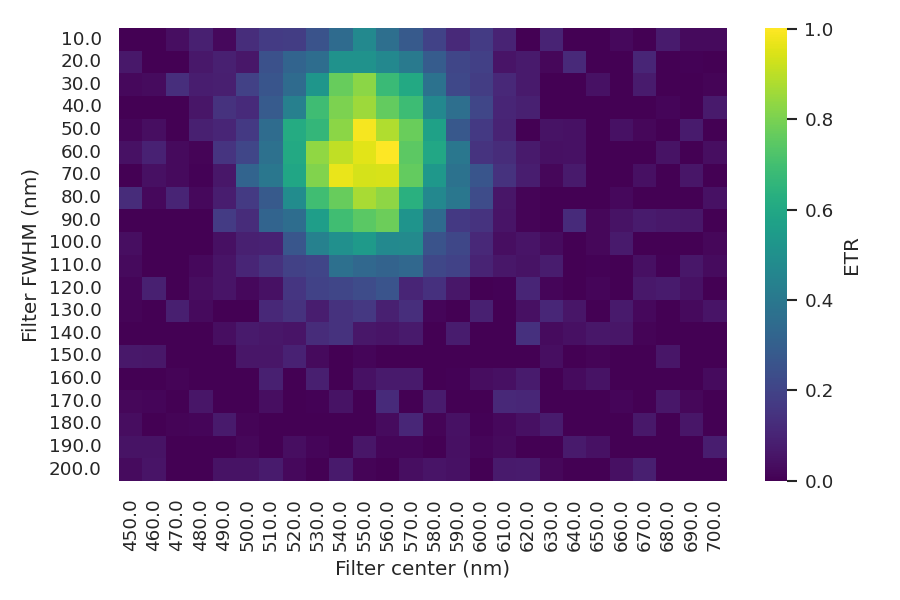
\includegraphics[width=\textwidth]{figures/heatmap_etr.png}
    \subcaption{ETR per absorbed photon heatmap (filter centre vs FWHM).}
\end{minipage}\hfill
\begin{minipage}{0.49\textwidth}
    \centering
    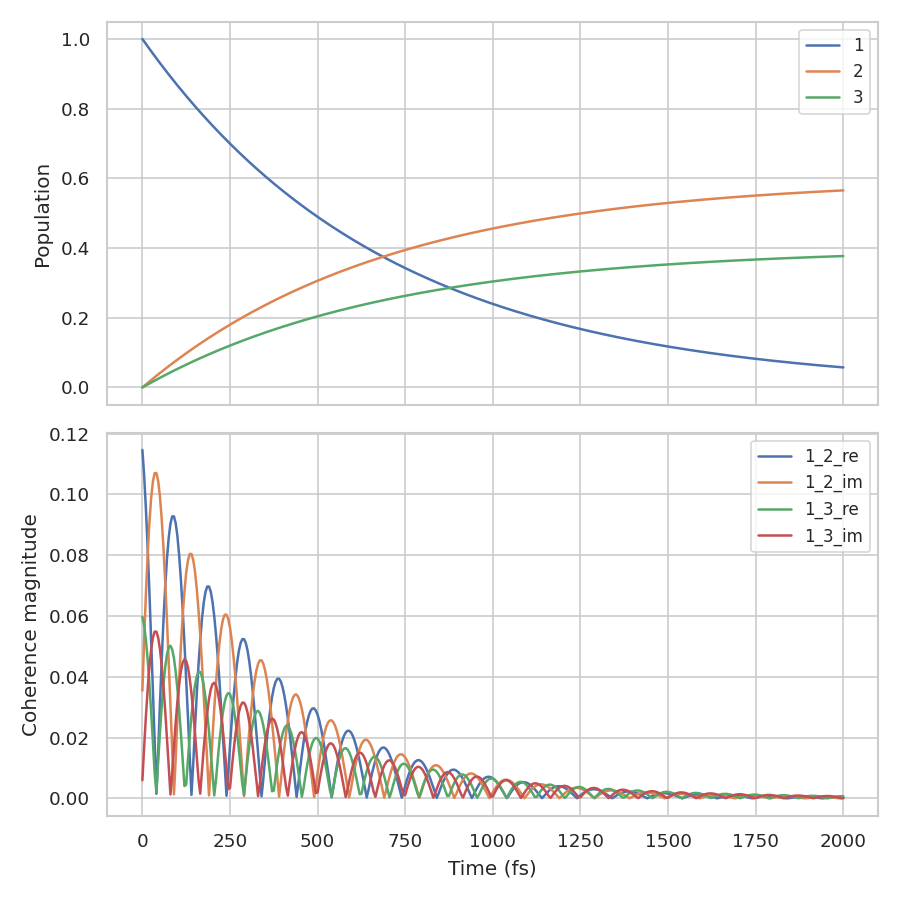
\includegraphics[width=\textwidth]{figures/traces.png}
    \subcaption{Time-domain traces: site populations and coherence magnitudes.}
\end{minipage}

\begin{minipage}{0.49\textwidth}
    \centering
    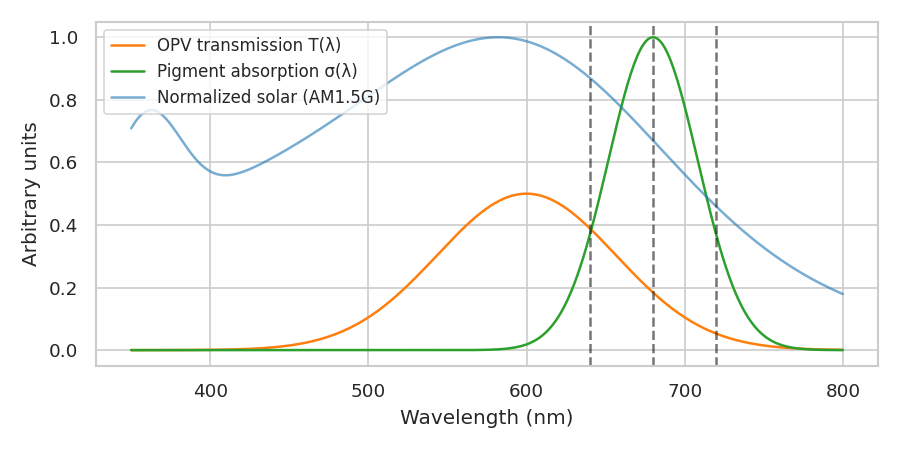
\includegraphics[width=\textwidth]{figures/overlay.png}
    \subcaption{Spectral overlay: $T(\lambda)$, $\sigma(\lambda)$ and solar spectrum.}
\end{minipage}\hfill
\begin{minipage}{0.49\textwidth}
    \centering
    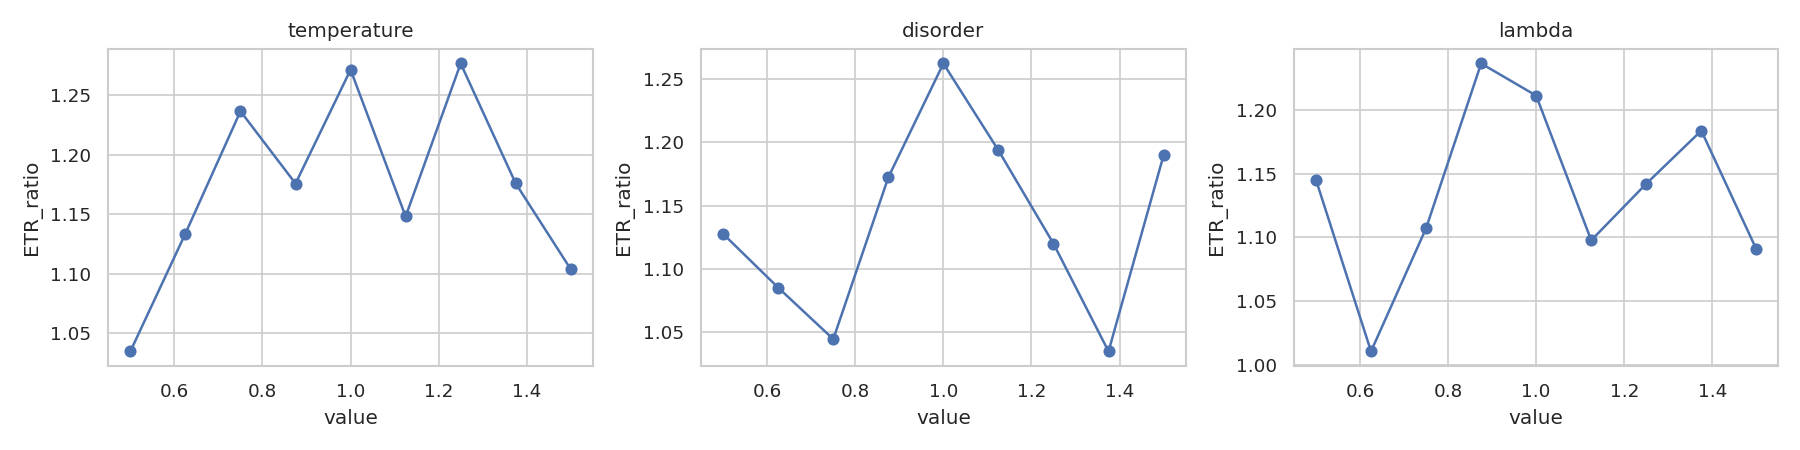
\includegraphics[width=\textwidth]{figures/robustness.png}
    \subcaption{Robustness panels: sensitivity to temperature, disorder and coupling.}
\end{minipage}

\caption{Summary of numerical results: (a) heatmap of ETR per absorbed photon as a function of filter centre wavelength and filter FWHM; (b) representative time-domain traces of site populations and off-diagonal coherence magnitudes $|\mathtt{\rho}_{ij}(t)|$ for exemplar filter choices; (c) overlay of OPV transmission $T(\omega)$, pigment absorption $\sigma(\omega)$ and vibronic mode positions; (d) robustness analysis.}
\label{fig:placeholders}
\end{figure*}

\subsection*{Practical scenarios and impact estimation}

To translate our quantum-dynamical findings into practical agrivoltaic metrics we construct a simple scenario model. For a given OPV transmission $T(\omega)$ and panel packing fraction $f_{\rm panel}$ (fraction of ground area covered), the incident PAR available to the crop is reduced to $f_{\rm panel}\,\Phi_{\rm PAR}^{\rm trans}$. Here we define
\begin{equation*}
\Phi_{\rm PAR}^{\rm trans}=\int_{\lambda_{400}}^{\lambda_{700}} d\lambda\,T(\lambda)\,I_{\rm solar}(\lambda).
\end{equation*}
The crop-level productivity change $\Delta Y$ (e.g., \si{\kilogram\per\hectare\per\yr}) is estimated via a simplified light-response curve:
\begin{equation}
\Delta Y \approx Y_{\rm base}\left(\frac{\mathrm{ETR}_{\rm ph}(T)}{\mathrm{ETR}_{\rm ph}(\mathrm{baseline})}\right) - \Delta_{\rm shading},
\end{equation}
where $Y_{\rm base}$ is baseline yield under full sun, $\mathrm{ETR}_{\rm ph}(T)$ is the ETR per photon predicted under transmission $T$, and $\Delta_{\rm shading}$ captures yield loss due to reduced total PAR (parameterised from field studies \cite{Scarano2024, Adeyemi2025}). This coarse model permits estimation of cross-over points where improved light quality (higher ETR per photon) compensates for reduced PAR, informing practical OPV spectral design trade-offs. Full parameter values and worked examples are provided in the Supplementary Information.


\section*{Data availability}

All numerical data (Hamiltonians, spectral densities, transmission functions $T(\omega)$ used in parameter sweeps, and resulting time series for populations and coherences) that support the plots and findings of this study are available in the Supplementary Information. Input files for the \texttt{MesoHOPS} simulations and example scripts to reproduce principal figures will be deposited in a public repository (Zenodo/GitHub) and are available from the corresponding author upon reasonable request. A permanent DOI for the repository will be provided in the final manuscript.

\section*{Code availability}

The \texttt{adHOPS} implementation used is the open-source \texttt{MesoHOPS} library (see \cite{Citty2024}) and simulations were run with version and commit hashes documented in the Supplementary Information. Analysis scripts used to post-process trajectories and compute ETR and coherence metrics will be provided in the public repository referenced above.

\section*{Author contributions}

T.F.G. developed the quantum dynamical modelling framework, performed the \texttt{adHOPS} simulations and prepared the manuscript. J.-P.T.N. performed DFT-based parameterisation, contributed to the agrivoltaic modelling and the interpretation of agricultural implications. S.G.N. conceived the project, assisted with the electronic structure aspects and supervized all the project. All authors discussed the results and contributed to revising the manuscript.

\section*{Competing interests}
The authors declare no competing interests.

\section*{Acknowledgements}
This work was supported by [funding sources to be inserted]. The authors thank [colleagues and facilities to be inserted] for helpful discussions and for providing the MesoHOPS code base. Computational resources were provided by [institutional cluster, to be inserted].

% Use the local consolidated bibliography file(s). BibTeX will be run below.
\bibliography{Ref_HOPS}

\end{document}
